\documentclass{article}
    % General document formatting
    \usepackage[margin=0.7in]{geometry}
    \usepackage[parfill]{parskip}
    \usepackage{amsopn}
    \usepackage{mathtools}
    \usepackage[utf8]{inputenc}
    \usepackage{hyperref}
    \usepackage{multicol}
    \usepackage{amsmath,amssymb,amsfonts,amsthm}
    \usepackage{dot2texi}
    \usepackage{tikz}
    \usepackage{mdframed}
    \usepackage[section]{placeins}
    \usetikzlibrary{shapes,arrows}

    \DeclareMathOperator{\StringT}{StringT}
    \DeclareMathOperator{\NumberT}{NumberT}
    \DeclareMathOperator{\BooleanT}{BooleanT}
    \DeclareMathOperator{\LitT}{LitT}
    \DeclareMathOperator{\JSLit}{JSLit}
    \DeclareMathOperator{\JSTypeof}{JSTypeof}
    \DeclareMathOperator{\RecT}{RecT_\Gamma}
    \DeclareMathOperator{\ObjT}{ObjT_\Gamma}
    \DeclareMathOperator{\ListT}{ListT_\Gamma}
    \DeclareMathOperator{\SetT}{SetT_\Gamma}
    \DeclareMathOperator{\MapT}{MapT_\Gamma}
    \DeclareMathOperator{\ObjType}{ObjType}
    \DeclareMathOperator{\UnionT}{UnionT_\Gamma}
    \DeclareMathOperator{\InterT}{InterT_\Gamma}
    \DeclareMathOperator{\LookupObjRef}{\Gamma}
    \DeclareMathOperator{\String}{String}
    \DeclareMathOperator{\Number}{Number}
    \DeclareMathOperator{\Boolean}{Boolean}
    \DeclareMathOperator{\type-ref}{ref}
    \DeclareMathOperator{\Type}{{Type_\Gamma}}
    \DeclareMathOperator{\NoSuper}{NoSuper}
    \DeclareMathOperator{\InterOrObj}{InterOrObj}
    \DeclareMathOperator{\ObjectSubtype}{ObjectSubtype_\Gamma}
    \DeclareMathOperator{\RecordSubtype}{RecordSubtype}
    \DeclareMathOperator{\Value}{Value_{\Gamma, \Sigma}}
    \DeclareMathOperator{\StringV}{StringV}
    \DeclareMathOperator{\NumberV}{NumberV}
    \DeclareMathOperator{\BooleanV}{BooleanV}
    \DeclareMathOperator{\RecV}{RecV_{\Gamma, \Sigma}}
    \DeclareMathOperator{\ObjV}{ObjV_{\Gamma, \Sigma}}
    \DeclareMathOperator{\ListV}{ListV_{\Gamma, \Sigma}}
    \DeclareMathOperator{\SetV}{SetV_{\Gamma, \Sigma}}
    \DeclareMathOperator{\MapV}{MapV_{\Gamma, \Sigma}}
    \DeclareMathOperator{\UnionV}{UnionV_{\Gamma, \Sigma}}
    \DeclareMathOperator{\ValueType}{ValueType_{\Gamma, \Sigma}}
    \DeclareMathOperator{\textref}{ref}
    \DeclareMathOperator{\ObjFields}{ObjFields}
    \DeclareMathOperator{\ObjPairsMatch}{ObjPairsMatch}
    \DeclareMathOperator{\where}{ where }
    \DeclareMathOperator{\textif}{ if }
    \DeclareMathOperator{\suchthat}{s.t.}
    \newcommand{\ValueRef}{\textref}
    \newcommand{\ValueDeref}[1]{\Sigma(#1)}
    \newcommand{\subtype}{<:_\Gamma}
\begin{document}

\title{Sinap's Type System}
\author{Sheyne Anderson}
\maketitle
\section{Intro}
Sinap IDE is a program to allow editing of graph
programs in various graph programming langauages. Each of these 
languages is loaded into Sinap as a ``plugin" and is 
referred to as an interpreter. More information 
about the editor can be found at 
\href{https://2graphic.github.io}{2graphic.github.io}.
Because the goal of Sinap IDE is to be an editor for many 
different graph-languages we designed the user interface (UI)
to change to best support the plugin that is currently loaded. 

The idea is that while editing a graph, components of the
graph will have different attributes associated with them 
that the editor should present contextually. For example, in
a graph-language describing deterministic finite-state 
automata (DFAs) edges should have a ``symbol" attribute of 
type character corresponding to the input by which this 
edge should be followed. 

\begin{figure}
    \centering
    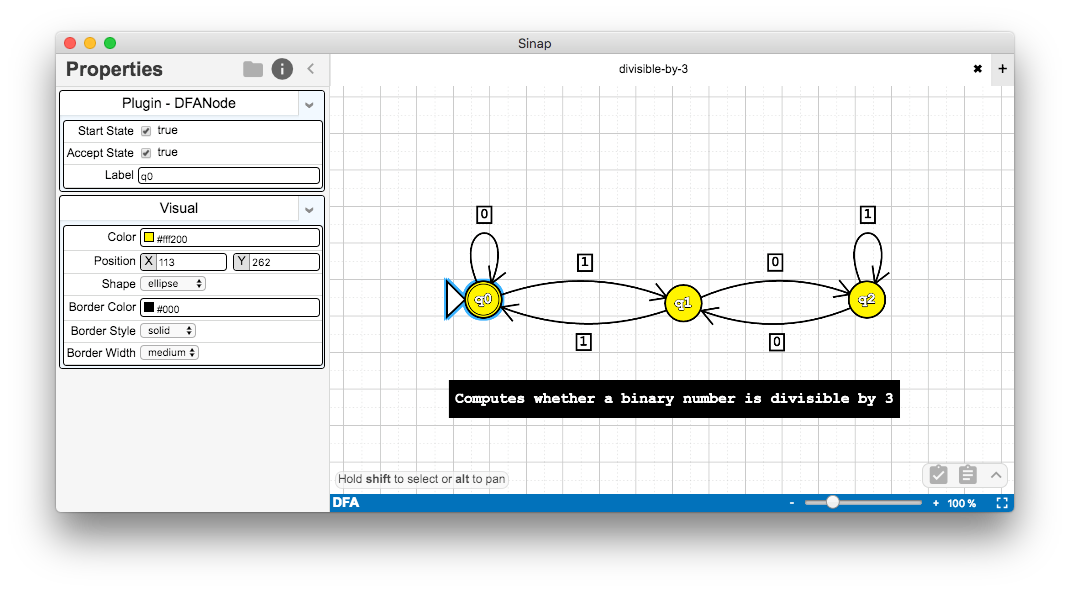
\includegraphics[width=.8\textwidth]{sinap-screenshot}
    \caption{Sinap IDE editing a graph}
    \label{sinap-screenshot}  
\end{figure}

As you can see in Figure \ref{sinap-screenshot}, Sinap's UI
presents the user with nodes and edges which can be selected 
and edited in the sidebar. Allowing the sidebar to change based
on which interpreter is loaded is the purpose of Sinap's Type System. 
This document presents a model for the type system. 
    
Sinap's Type System consists of two parts:

\begin{enumerate}
    \item A data-language to describe graph components 
    (implemented in values.ts)
    \item A data-description language to define valid schema 
    (implemented in types.ts)
    for the data language
\end{enumerate}

The code for both can be found at 
\href{https://github.com/2graphic/sinap-types}
{github.com/2graphic/sinap-types}.

The data that are allowable in the sidebar can be more complicated than
simple strings and numbers. Figure \ref{sinap-screenshot}, the ``Position" attribute
of the node has a structure that similar to the following TypeScript code:

\begin{samepage}
\begin{verbatim}
type Point = {
    x: number;
    y: number;
}
\end{verbatim}
\end{samepage}

Complex types aren't limited to fields directly on nodes and edges,
and can be arbitrarily nested. 

The goal of creating Sinap's Type System is to allow interpreter 
implementers to specify what 
kinds of graphs are valid for their interpreter. This means that 
the interpreter specifies the various fields on nodes and edges 
and can assume that those fields are present on all of the graph elements
that it receives. It also allows different kinds of nodes and edges to
exist in the same graph and allows for rules defining what kinds of
nodes can connect to which edges. 

\section{Types}

\subsection{Notation}

The symbol \((\operatorname{Kind}_1, ...)\) is equivalent to 
\((\operatorname{Kind}_i)\). They are also equivalent to 
\((\operatorname{Kind}_1, ..., \operatorname{Kind}_n)\)
where \(n\) is unspecified and represent an ordered list 
of \(n\) elements. \(\{\operatorname{Kind}_i\}\) represents 
the set of the elements of the list. 

``\(\_\)'' represents a symbol that has been omitted for brevity.

\subsection{Type Model}
The data-description language is called Sinap Types. There are 
several kinds of types:

\begin{itemize}
    \item \(\LitT(\JSLit)\) is the type for literal primitives, specifically,
    string, number, and boolean literals. 
    Examples include \(\LitT(17), \LitT(\text{``Hello"}), \text{ and } 
    \LitT(false)\). A value will match this type if and only if it is
    exactly the value of the literal in the type. 
    \item \(\StringT\) is a type matching all strings.
    \item \(\NumberT\) is a type matching all numbers.
    \item \(\BooleanT\) is a type matching all booleans.
    \item \(\RecT((\String, \Type)...)\) is a type for records. 
    The arguments come in pairs of \((\String, \Type)\) where
    \(\String\) is the name of some field and \(\Type\) is the
    type of that field.
    \item \(\ListT(\Type)\) is a type for homogeneous lists. The
    parameter is the type of all the elements of the list. 
    \item \(\SetT(\Type)\) is a type for an unordered collection
    of elements of type \(\Type\).
    \item \(\MapT((\Type)_1, (\Type)_2)\) is the type of a mapping from 
    \((\Type)_1\) to \((\Type)_2\).
    \item \(\ObjT(\String, \String | \NoSuper, ((\String, \Type), ...))\)
    describes an object type. Its name is the first argument, 
    its super-type is the second argument, and the new fields 
    it introduces is the tuple of (key, value) pairs that form the
    last argument. 
    \item \(\InterT(\ObjT,  ...)\) is the intersection of several 
    object types and acts like a single object type with all the 
    properties of the intersected types. 
    \item \(\UnionT(\Type, ...)\) is a union of several types. 
    Values with this type act as a collection with a single element
    whose type is one of the \(\{(\Type)_i\}\). In Sinap, a drop down 
    menu that allows ``Narrow'', ``Wide'', or some number would be 
    typed as \(\UnionT(\LitT(``\text{Narrow}"), \LitT(``\text{Wide}"),
     \NumberT)\).
\end{itemize}

These informal descriptions of the various types is recognized formally 
in Figure \ref{sinap-types-model}.

\begin{figure}
\begin{mdframed}
\begin{align*}
\begin{aligned}
\Type = &\LitT(\JSLit) \\
&|\StringT \\
&|\NumberT \\
&|\BooleanT \\
&|\RecT((\String, \Type), ...) \\
&|\ListT(\Type) \\
&|\SetT(\Type) \\
&|\MapT(\Type, \Type) \\
&|\ObjT\left(\begin{aligned}
    &\String, \String | \NoSuper, \\
&((\String, \Type), ...)
\end{aligned}\right) \\
&|\InterT(\ObjT, ...) \\
&|\UnionT(\Type, ...)\\
\end{aligned}
\quad\quad\quad\begin{aligned}        
\begin{aligned}
\JSLit = &\operatorname{JSString} \\
&| \operatorname{JSNumber} \\
&| \operatorname{true} \\
&| \operatorname{false} \\
\end{aligned}\\\\
\begin{aligned}
\JSTypeof(\operatorname{JSString}) &= \StringT \\
\JSTypeof(\operatorname{JSNumber}) &= \NumberT \\
\JSTypeof(\operatorname{true}) &= \BooleanT \\
\JSTypeof(\operatorname{false}) &= \BooleanT \\
\end{aligned}  
\end{aligned}  
\end{align*}
\end{mdframed}
\caption{Formal Description of Sinap Types}
\label{sinap-types-model}
\end{figure}

\subsection{Subtype Relations}

With types defined, it is necessary to define a subtype 
relation (\(\bullet\subtype\bullet\)). Subtypes correspond 
roughly to the idea that if \(A\subtype B\) then \(A\)
can be used where \(B\) can be used. The subtype relation,
as formally described in Figures \ref{subtype-definitions} and \ref{subtype-helpers}, 
defines literals as subtypes of their respective general types.
For example \(\LitT(\text{``Hello"})\subtype\StringT\). It defines
record subtypes structurally; that is, all the supertype's fields 
are present in the subtype and the types of these fields in the subtype
are subtypes of the corresponding fields in the supertype. 
Objects are subtyped nominally, meaning that the supertype must be
found somewhere in the subtype's inheritance chain. Unions are
subtypes of other unions as long as all of the types in the 
subtype are subtypes of some type in the supertype. Intersections are 
subtypes of other intersections if all the supertype's elements are 
subtypes of all the elements of the suptertype. Additionally, 
intersections are subtypes of objects that they contain. Lists, 
Sets, and Maps are subtypes if their arguments are subtypes. This
approach to collections is widespread and used in languages such
as Java. It is technically not sound when paired with mutation 
but works well most of the time in practice. \(\Gamma\) is an 
argument to the subtype relation, so it can be threaded through 
to object types, which use it to lookup supertypes by name. 

\begin{figure}
\begin{mdframed}        
\begin{align*}
    (\Type)_1&\subtype(\Type)_1 \\
    \LitT(\JSLit_1)&\subtype(\Type)_1 &&\textif \JSTypeof(\JSLit_1) = (\Type)_1 \\
    \UnionT((\Type)_{1,1}, ...)&\subtype\UnionT((\Type)_{2,1}, ...) 
    &&\textif \forall T\in \{(\Type)_{1,i}\} \exists T' \in \{(\Type)_{2,i}\} \suchthat T\subtype T' \\
    \InterT((\Type)_{1,1}, ...)&\subtype\InterT((\Type)_{2,1}, ...) 
    &&\textif \forall T\in \{(\Type)_{1,i}\} \forall T' \in \{(\Type)_{2,i}\} T\subtype T' \\
    \InterT(..., (\Type)_i, ...)&\subtype\ObjT_1 &&\textif (\Type)_i\subtype\ObjT_1  \\
    \ObjT_1 &\subtype \ObjT(\String_1, \_, \_) &&\textif \ObjectSubtype(\String_1, \ObjT_1)\\
    \RecT_1&\subtype\RecT_2 &&\textif \RecordSubtype(\RecT_1, \RecT_2) \\
    \ListT((\Type)_1)&\subtype\ListT((\Type)_2) &&\textif (\Type)_1\subtype(\Type)_2 \\
    \SetT((\Type)_1)&\subtype\SetT((\Type)_2) &&\textif (\Type)_1\subtype(\Type)_2 \\
    \MapT((\Type)_{11}, (\Type)_{12})&\subtype\MapT((\Type)_{21}, (\Type)_{22}) &&\textif (\Type)_{11}\subtype(\Type)_{21} \text{ and } (\Type)_{12}\subtype(\Type)_{22} \\
\end{align*}
\end{mdframed}        
\caption{Definition of the subtype relation (\(\bullet\subtype\bullet\))}
\label{subtype-definitions}
\end{figure}
\begin{figure}
\begin{mdframed}        
\begin{align*}
    \ObjectSubtype(\String_1, \ObjT(\String_2,\_, \_)) \quad &\textif 
    \quad (\String_1 = \String_2)\\
    \ObjectSubtype(\String_1, \ObjT(\_,\String_2, \_)) \quad &\textif 
    \quad \ObjectSubtype(\String_1, \LookupObjRef(\String_2)))
\end{align*}
\begin{align*}
    \RecordSubtype &\left(\begin{aligned}
        &\RecT((\String_{1,1}, (\Type)_{1, 1}), ..., (\String_{1,n}, (\Type)_{1, n})), \\
        &\RecT((\String_{2,1}, (\Type)_{2, 1}), ..., (\String_{2,m}, (\Type)_{2, m}))
    \end{aligned}\right) \\
    &\textif \{\String_{2,i}\} \subset \{\String_{1,i}\} \text{ and } \String_{1, i} = \String_{2, j} \implies (\Type)_{1, i} \subtype (\Type)_{2, j}
\end{align*}
\end{mdframed}        
    \caption{Helper meta-functions for the subtype relation}
\label{subtype-helpers}
\end{figure}

While Sinap's Type System is implemented as a library and can have 
concrete syntaxes in several languages, our most mature implementation 
is in TypeScript. 

An example of how TypeScript can be converted into this form is given in 
Figures \ref{types-example} and \ref{types-example-code}. 

\begin{figure}
\begin{mdframed}
\begin{align*}
    \text{Nodes} = &\UnionT\left(
        \begin{aligned}
        &\ObjT\left(
            \begin{aligned}    
                \text{``Node1"}, \NoSuper, \left(
                    \begin{aligned}
                        &(\text{``label"}, \StringT),  \\
                        &(\text{``customAttribute"}, \NumberT)
                    \end{aligned}\right)
            \end{aligned}\right),  \\
        &\ObjT\left(\text{``Node2"}, \NoSuper, \left(\begin{aligned}
            (&\text{``label"}, \StringT),  \\
            (&\text{``otherAttribute"}, \RecT\left(
                \begin{aligned}
                    (&\text{``f1"}, \BooleanT),  \\
                    (&\text{``f2"}, \NumberT)
                \end{aligned}\right)
        \end{aligned}\right)\right)
        \end{aligned}\right)  \\
    \text{Edges} = &\UnionT\left(\ObjT\left(
        \text{``Edge"}, \NoSuper,  
        \left(\begin{aligned}
            (&\text{``label"}, \StringT), \\
            (&\text{``source"}, \ObjT(\text{``Node1"}, \_, \_)), \\
            (&\text{``destination"}, \ObjT(\text{``Node2"}, \_, \_)) \\             
        \end{aligned}\right)\right)\right)
\end{align*}
\end{mdframed}
\caption{An example of an interpreter's description of valid graphs}
\label{types-example}
\end{figure}

\begin{figure}
\begin{mdframed}    
\begin{multicols}{2}
\begin{verbatim}
class Node1 {
    label: string;
    customAttribute: number;
}

class Node2 {
    label: string;
    otherAttribute: {
        f1: boolean,
        f2: number
    };
}

class Edge {
    label: string
    source: Node1;
    destination: Node2;
}

type Nodes = Node1 | Node2;
type Edges = Edge;
\end{verbatim}
\end{multicols}
\end{mdframed}
\caption{TypeScript code to go with Figure \ref{types-example}}
\label{types-example-code}
\end{figure}

\section{Values}

Now that we have a description of valid graph structures for some
interpreter, we need to define a language for describing specific 
graphs. 

Note that Values are parameterized by \(\Sigma\), a ``store" that
allows Values to reference other Values without including their 
whole structure. This allows for cycles. 

\textbf{TODO: specifically \(\Sigma\) maps refs to values}
\begin{figure}
\begin{mdframed}
\begin{align*}
    \Value =& \StringV((\Type)_1, \String_1) \quad\where (\Type)_1 \subtype \StringT \\
    &| \NumberV((\Type)_1, \Number_1) \quad\where (\Type)_1 \subtype \NumberT \\
    &| \BooleanV((\Type)_1, \Boolean_1) \quad\where (\Type)_1 \subtype \BooleanT \\
    &| \ObjV((\Type)_1, V=((\String_1, \ValueRef_1]), ...)) \quad\where 
    \ObjPairsMatch(\ObjFields((\Type)_1), V) \\
    &| \UnionV(\UnionT(..., (\Type)_i, ...), \ValueRef_1) \where
    \ValueType(\ValueRef_1) \subtype (\Type)_i\\
    &| \ListV(\ListT((\Type)_1), (\ValueRef_1, ...)) \where \ValueType(\ValueRef_i) \subtype (\Type)_1 \\
    &| \SetV(\SetT((\Type)_1), \{\ValueRef_1, ...\}) \where \ValueType(\ValueRef_i) \subtype (\Type)_1 \\
    &| \MapV(\MapT((\Type)_1, (\Type)_2), ((\ValueRef_{1,1}, \ValueRef_{2,1}), ...)) \where \bigwedge
    \begin{aligned}
        \ValueType(\ValueRef_{1, i}) \subtype (\Type)_1 \\
        \ValueType(\ValueRef_{2, i}) \subtype (\Type)_2 
    \end{aligned}\\
\end{align*}

\begin{align*}
    \ObjFields(\ObjT(\_, \String_S, (P_1 = (\String_1, (\Type)_1), ...))) &= \operatorname{concat}(\ObjFields(\LookupObjRef(\String_S), (P_n))) \\
    \ObjFields(\InterT(ObjT_1, ...)) &= \operatorname{concat}(\ObjFields(\ObjT_1), ...)
\end{align*}

\begin{align*}
    \ValueType(\ValueRef_1) &= \ValueType(\ValueDeref{\ValueRef_1}) \\
    \ValueType(\StringV((\Type)_1, \_)) &= (\Type)_1 \\
    \ValueType(\NumberV((\Type)_1, \_)) &= (\Type)_1 \\
    \ValueType(\BooleanV((\Type)_1, \_)) &= (\Type)_1 \\
    \ValueType(\ObjV((\Type)_1, \_)) &= (\Type)_1 \\
    \ValueType(\UnionV((\Type)_1, \_)) &= (\Type)_1 \\
    \ValueType(\ListV((\Type)_1, \_)) &= (\Type)_1 \\
    \ValueType(\SetV((\Type)_1, \_)) &= (\Type)_1 \\
    \ValueType(\MapV((\Type)_1, \_)) &= (\Type)_1 \\
\end{align*}
\begin{align*}
    \ObjPairsMatch(((\String_1, (\Type)_1),...), ((\String_1, \ValueRef_1), ...)) 
    \textif \forall i, \ValueType(\Value_i) \subtype (\Type)_i
\end{align*}
\end{mdframed}
\caption{Definition of Value}
\label{value-definition}
\end{figure}

A valid graph then matches 
\[(\ListV(\ListT(\textit{Nodes}), \_), \ListV(\ListT(\textit{Edges}), \_))\]
for some appropriate definition of \textit{Nodes} and \textit{Edges}.

\subsection{Example}
\begin{figure}
    \centering
    \begin{dot2tex}[dot, scale=0.5]
    digraph {
        "Start Node" -> "End Node";
    }
    \end{dot2tex}
    \caption{A simple graph}
    \label{simplegraph}
\end{figure}   
To give an example, the simple graph given in Figure \ref{simplegraph} 
might be modeled as is shown in Figure \ref{values-example1}.
The values loaded into \(\Sigma\) in Figure \ref{values-example1} can probably 
better be understood Figure \ref{values-example2}.

\newcommand{\treeDraw}[2]{#1 \left(\begin{aligned} &#2\end{aligned}\right)}
\newcommand{\treeNext}{,\\&}
\newcommand{\valRef}[1]{\ValueRef_\textit{#1}}
\newcommand{\textq}[1]{\text{``#1"}}

\begin{figure}
\begin{mdframed}
\begin{align*}
    \Sigma(\valRef{0O})&=\ObjV(\ObjT_0, ())\\ 
    \Sigma(\valRef{0U})&=\UnionV(\UnionT_0, \valRef{0O})\\
    \Sigma(\valRef{1S})&=\treeDraw\StringV{\StringT_1, \textq{Start Node}}\\
    \Sigma(\valRef{1O})&=\treeDraw\ObjV{\ObjT_1,\treeDraw{}{
        (\textq{label}, \valRef{1S})\treeNext
        (\textq{destination}, \valRef{3U})
        }}\\
    \Sigma(\valRef{1U})&=\treeDraw\UnionV{\UnionT_1, \valRef{1O}}\\
    \Sigma(\valRef{2S})&=\treeDraw\StringV{\StringT_2, \textq{End Node}}\\
    \Sigma(\valRef{2O})&=\treeDraw\ObjV{\ObjT_2,\treeDraw{}{
        (\textq{label}, \valRef{2S})\treeNext
        (\textq{destination}, \text{nil})
        }}\\
    \Sigma(\valRef{2U})&=\treeDraw\UnionV{\UnionT_2, \valRef{2O}}\\
    \Sigma(\valRef{3O})&=\treeDraw\ObjV{\ObjT_3,\treeDraw{}{
        (\textq{children}, \valRef{4})
        }}\\
    \Sigma(\valRef{3U})&=\treeDraw\UnionV{\UnionT_3, \valRef{3O}}\\
    \Sigma(\valRef{4})&=\treeDraw\ListV{\ListT_4, (\valRef{2U})}\\
    \textit{Nodes}_1 &= \treeDraw\ListV{\ListT_5, (\valRef{1U}, \valRef{2U})} \\
    \textit{Edges}_1 &= \treeDraw\ListV{\ListT_6, (\valRef{3U})} \\
\end{align*}
\end{mdframed}
\caption{}
\label{values-example1}
\end{figure}

\begin{figure}
    \centering
    \begin{dot2tex}[fdp, scale=0.5]
    digraph {
        "1U" [label="UnionV (1U)"];
        "2U" [label="UnionV (2U)"];
        "3U" [label="UnionV (3U)"];
        "1O" [label="ObjV (1O)"];
        "2O" [label="ObjV (2O)"];
        "3O" [label="ObjV (3O)"];
        "1S" [label="StringV (1S)"];
        "2S" [label="StringV (2S)"];
        "3S" [label="StringV (3S)"];
        "4" [label="ListV (4)"];
        "1U" -> "1O";
        "1O" -> "1S" [label="label"];
        "2U" -> "2O" [label="label"];
        "2O" -> "2S";
        "3U" -> "3O";
        "3O" -> "3S";
        "1O" -> "3U" [label="destination"];
        "2O" -> "0U" [label="destination"];
        "3O" -> "4" [label="children"];
        "4" -> "2U"
    }
    \end{dot2tex}
\caption{A diagram of the example Values}
\label{values-example2}
\end{figure}

\section{Conclusion}

Sinap types is useful for generically describing data-structures 
so that GUIs for their entry can be automatically generated. We implemented the 
above as a TypeScript library that gives runtime access to the types 
of all values used. We implemented loaders to build the type information 
for this library from TypeScript source code and to build it dynamically from 
Python. This allows Sinap Plugins to be built in Python or TypeScript. 
The TypeScript implementation is especially powerful because essentially 
no thought needs to be given to Sinap IDE while writing an interpreter. 

When using the Sinap Type-System for to create the IDE we added 
some invariants to specialize the Type System to graphs. 
\begin{enumerate}
    \item There must be types Nodes and Edges which are unions of \(\ObjT\) subtypes. 
    \item If any Edge type specifies ``source'' or ``destination'', it must be a Node subtype
    and its type will be respected and added as a constraint when creating graphs.
    \item The same goes for Nodes, except that the names are ``children'' and 
    ``parents'' and the types have to be lists of edges.
\end{enumerate}

This allows programmers writing interpreters to access connectivity information, 
a critical element of creating a graph interpreter. 

\end{document}
